%
%%
%% file: recombination.tex
%%
%

% =======================================================================
	\subsection{Recombination\index{recombination}}
% =======================================================================

After the individuals have been selected for reproduction they mate by
recombining their respective chromosomes.  Depending on the
representation of the chromosome different
recombination\index{recombination!operator} operators can be applied. The most
universal operator is the \emph{crossing over} which is, in principle,
applicable for all chromosomes which can be described by a sequence of
values.  This is the standard recombination operator in GAs.  The
recombination of continuous values, as needed in ESs, is introduced in
\secref{recombination:subsubs:recombinationOfContinuesValues}.


% -----------------------------------------------------------------------
	\subsubsection{Crossover of Strings}
% -----------------------------------------------------------------------

In most GAs, individuals are represented by fixed-length strings of
symbols of a finite alphabet.
Recombination is implemented by means of crossing-over.
The crossover operator\index{crossover!operator} acts on pairs
of individuals (\myindex{parents}) and creates new individuals
(\myindex{offsprings}) by exchanging segments from the parents' strings.
The number and the position of these segments are determinded by the
crossover points\index{crossover!points}.
Usually these crossover points are sampled randomly.
As a constraint the granularity\index{crossover!granularity}
of crossover can be controlled so that
crossover points are not selected at any point within the string.
This may be useful if chunks of consecutive symbols encode single items which
should not be disrupted by crossover.
A comparison and analysis of the most popular methods to choose
crossover points is presented in \cite{Spears:91b}.
The probability of the application of the crossover operator is
controlled by the crossover rate.

% .......................................................................
	\paragraph{$m$-Point Crossover\index{crossover!$m$-point}}

The disruptiveness is controlled by the number of crossover points $m$.
Figure \ref{f:crossover} shows examples of one point and two point
crossover.

\begin{figure}[ht]
\centerline{
  \hfill
  (a)~~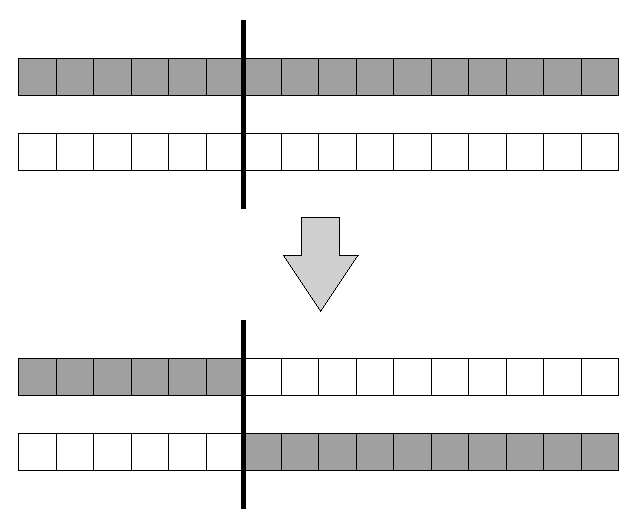
\includegraphics[width=0.3\columnwidth]{cross1.eps}
  \hfill
  (b)~~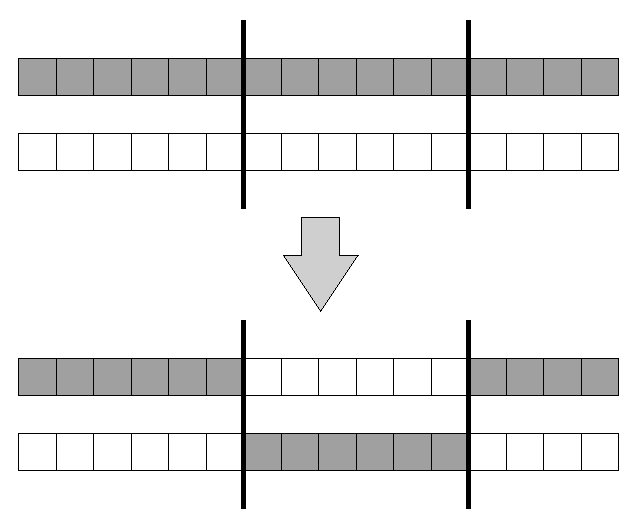
\includegraphics[width=0.3\columnwidth]{cross2.eps}
  \hfill
}
\caption[One point and two point crossover]{
  \label{f:crossover}
  (a) One point crossover.
  (b) Two point crossover.
}
\end{figure}
% .......................................................................
	\paragraph{Uniform Crossover\index{crossover!uniform}}

Syswerda \cite{Syswerda:89} defines a family of \emph{uniform}
crossover operators which produce offspring by randomly selecting at
each loci the allele of one of the parents.  This corresponds on
average to a ($L/2$)-point crossover on strings of length $L$. Uniform
crossover is an adaptation of Mendel's chance model to haploid
organisms \cite{Asoh:94}.



% \paragraph{Punctuated Crossover}
% Adaptive Crossover \cite{White:94}



% .......................................................................
	\paragraph{Multi-Parent Crossover\index{crossover!multi-parent}}

A multi-parent operator uses two or more parents to generate
offsprings. Gene scanning, as discussed in \cite{Eiben:94},
generalizes uniform-crossover to take more than two parents into
account. For each position in the offspring a parent is chosen to
contribute its allele. There are different methods to choose a parent.

\begin{itemize}

  \item Uniform scanning\index{scanning!uniform}. For each allele in the offspring a parent is
        chosen randomly.  Each parent has an equal chance of
        contributing an allele to be inherited by the offspring.

  \item Occurence-based scanning\index{scanning!occurence-based}. The allele which occurs most often
        is chosen for inheritance.

  \item Fitness-based scanning\index{scanning!fitness-based}. The probability of a parent to be
        selected is proportional to its fitness.

\end{itemize}



% -----------------------------------------------------------------------
	\subsubsection{Recombination of Continuous Values\index{recombination!continuous}}
	\label{recombination:subsubs:recombinationOfContinuesValues}
% -----------------------------------------------------------------------

In the field of ESs a variety of recombination operators have been
proposed, including sexual as well as panmictic operators.  In the
following the most frequently employed operators are shortly
introduced.


% .......................................................................
	\paragraph{Discrete Recombination\index{recombination!discrete}}

Discrete recombination means the same as uniform crossover, that is
for each allele one of the (two) parents is randomly selected for
inheritance.


% .......................................................................
	\paragraph{Intermediate Recombination\index{recombination!intermediate}}

In this form of recombination the new allele is a weighted sum of the
alleles of the corresponding parents.  In the simplest form this sum
is the arithmetic mean of all parent alleles.


% .......................................................................
	\paragraph{Panmictic Recombination\index{recombination!panmictic}}

Panmictic recombination involves more than two parents.  Combined with
discrete recombination this means that for each allele in the
offspring individual a parent is sampled anew.  In the case of
intermediate recombination each parent may contribute to the weighted
sum of alleles.
